% Section 7.2 - Results of Experiments 1 and 2 (Person 2)
% Numbers come ONLY from generated/exp2_numbers.tex and generated/exp2_tables.tex, which
% workload/exp2_summary.py writes from results/raw/ (make exp2 && make exp2-report).
% Until then every number prints as a bold "[run make exp2-report]" marker.
\providecommand{\exptwo}[1]{%
  \ifcsname exptwo@#1\endcsname\csname exptwo@#1\endcsname
  \else\textbf{[run make exp2-report]}\fi}
\InputIfFileExists{generated/exp2_numbers.tex}{}{}

\subsection{Results: normal operations and consistency tuning}\label{sec:results-exp2}

\paragraph{Method}
All measurements use the CassChat workload generator (\texttt{workload/runner.py}) in the
client container on the cluster network (Section~\ref{sec:setup}). The data-access layer
routes each request token-aware to a replica, disables driver retries
(\texttt{FallthroughRetryPolicy}) and speculative execution, and uses a 5\,s client timeout,
so every server-side failure is counted rather than hidden. Latency is measured in the
client around each request (\texttt{perf\_counter}) and logged with its outcome and
coordinator, one CSV row per operation. Fixed-rate runs are \emph{open loop}: requests are
scheduled every $1/\text{rate}$ seconds regardless of earlier responses
(200\,ops/s, 8 threads, 60\,s measured after a 10\,s warm-up that is not logged), for
each mode (write, read, mixed 50/50) and CL, repeated \exptwo{reps} times with the CL order
rotated between repetitions. Reads fetch the newest 10 messages of one of 100 rooms
preloaded with 10{,}000 messages. A closed-loop run per CL (32 threads, 30\,s) gives the
saturation throughput. The \emph{freshness probe} writes $\texttt{last\_seq} = n$ through
coordinator $A$ at CL $W$ and, as soon as the write is acknowledged, reads it through a
different coordinator $B$ at CL $R$; the read is stale if it returns less than $n$.

\paragraph{Experiment 1}
The committed Exp~1 evidence (\texttt{results/logs/exp1/}) shows the expected healthy
baseline: three nodes Up/Normal with one schema version and the Murmur3 partitioner; every
node owns 100\,\% of the data effectively; \texttt{getendpoints} lists all three
addresses for partition \texttt{general}; and a row written at QUORUM through cass1 was read
at ONE through cass3. The trace of that read shows the coordinator serving the row
locally and, through speculative retry, also from cass1 (Section~\ref{sec:consistency}).
The 60\,s baseline at QUORUM (mixed, 200\,ops/s) completed \exptwo{exp1-ops} operations
with \exptwo{exp1-err}\,\% errors at \exptwo{exp1-tput}\,ops/s; latency was
p50 \exptwo{exp1-p50}\,ms, p95 \exptwo{exp1-p95}\,ms and p99 \exptwo{exp1-p99}\,ms.

\paragraph{Latency and throughput}
Table~\ref{tab:exp2-grid} and Fig.~\ref{fig:exp2-latency} summarise the grid.
\exptwo{sentence-ordering} \exptwo{sentence-tail} \exptwo{sentence-errors}
\exptwo{sentence-rate} \exptwo{sentence-saturation}

\InputIfFileExists{generated/exp2_tables.tex}{}{%
  \begin{table}[t]\centering\footnotesize
  \caption{Experiment 2 results (generated by \texttt{make exp2-report}).}\label{tab:exp2-grid}
  \textbf{[run make exp2-report]}\end{table}}

\begin{figure}[t]\centering
\IfFileExists{../../results/figures/exp2_latency_percentiles.png}{%
  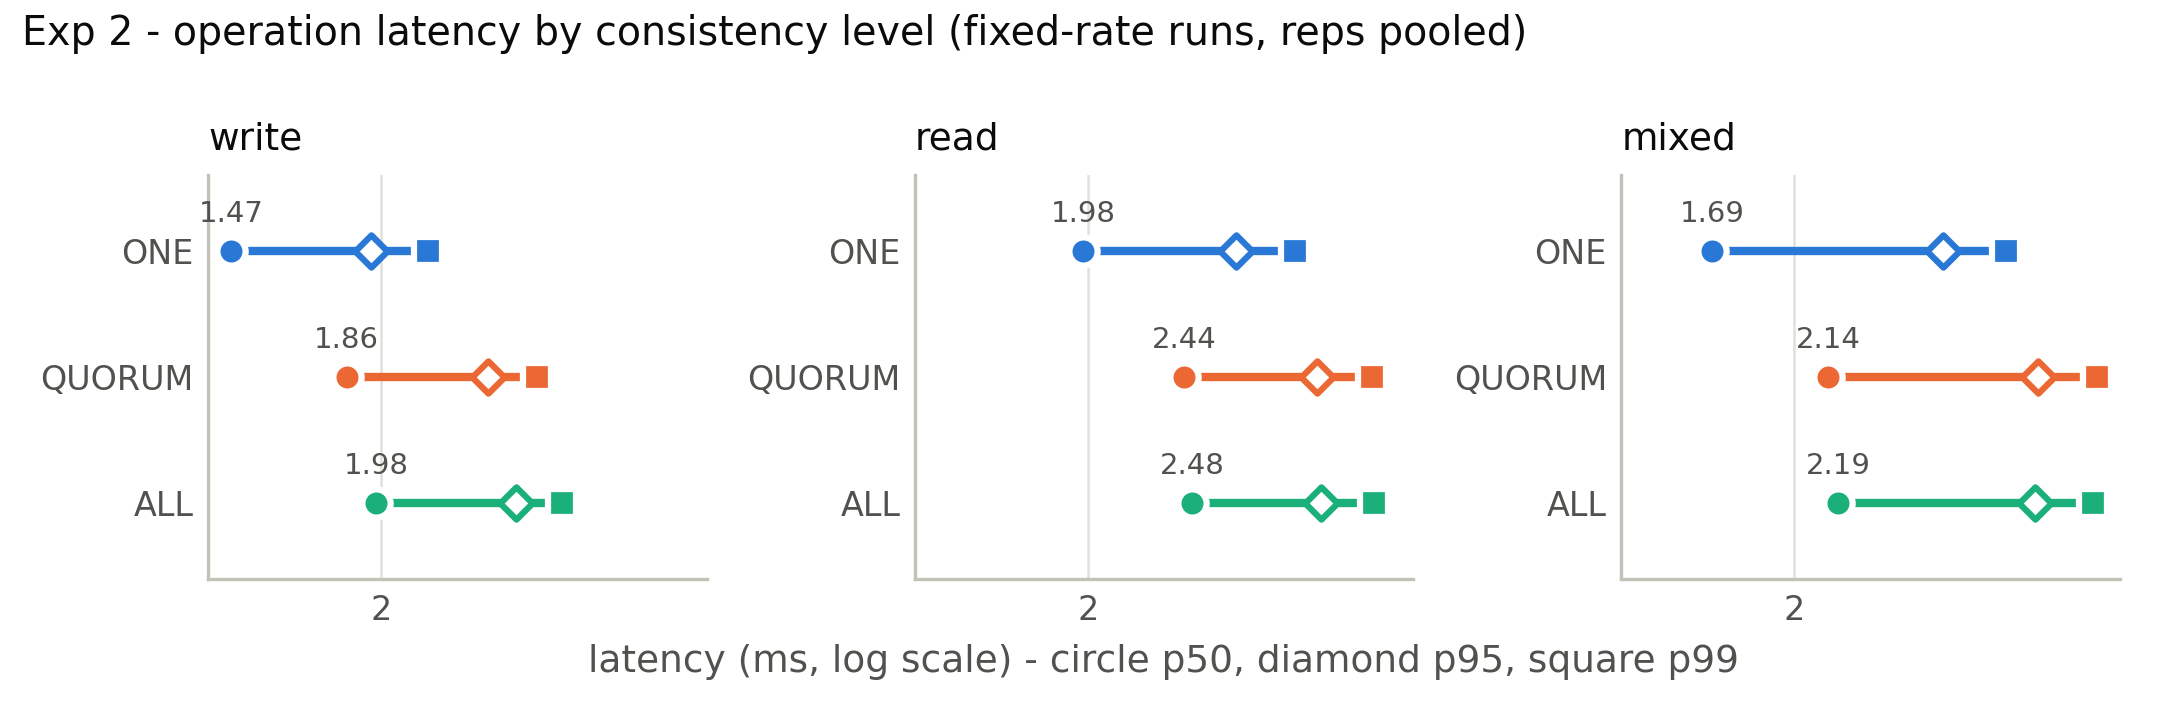
\includegraphics[width=\columnwidth]{exp2_latency_percentiles.png}}{%
  \fbox{\parbox{0.9\columnwidth}{\centering\vspace{8mm}\textbf{[run make exp2-report]}\vspace{8mm}}}}
\caption{Experiment 2: p50 (circle), p95 (diamond) and p99 (square) latency per consistency
level; fixed-rate runs, repetitions pooled.}\label{fig:exp2-latency}
\end{figure}

\paragraph{Freshness}
Table~\ref{tab:exp2-probe} lists the probe results. \exptwo{sentence-staleness}
The probe measures the most demanding case---a read issued within one client round trip of
the acknowledgement---so these rates are an upper bound for the steady-state workload, in
line with the PBS model~\cite{bailis2012pbs}.

\paragraph{Interpretation}
On a healthy cluster the price of a stronger level is latency, not availability: the
coordinator performs the same replication work for every write and only waits longer.
That price is small here because all replicas share one host and the replica round trip is
sub-millisecond; across racks or data centres the gap between ONE and ALL grows with the
slowest replica's distance, which is exactly the latency term of PACELC's ``else'' branch
(EL vs.\ EC)~\cite{abadi2012pacelc}. The \emph{availability} side of the trade-off appears
only when replicas fail: ALL rejects writes as soon as one replica is down, while QUORUM
keeps both reads and writes available and still overlaps (Exp~3 and Exp~5).

\paragraph{Threats to validity}
(i)~All nodes and the client share one machine, so network latency is unrealistically low
and CPU contention between containers can add noise; we recorded \texttt{docker stats}
during every run to rule out saturation. (ii)~The Python client is CPU-bound near
saturation, so closed-loop throughput is a lower bound on cluster capacity. (iii)~With a
bounded number of threads, an open-loop generator falls back to closed-loop behaviour if
all threads are busy; the runner reports operations that started more than 50\,ms late, and
such cells are rerun. (iv)~The working set fits in memtables and the page cache, so reads
rarely touch disk. (v)~The probe can detect staleness only within its own round trip;
a zero count means the inconsistency window was shorter than that, not that it does not
exist. (vi)~Three repetitions give limited statistical power; the table reports the
standard deviation of throughput across repetitions.
